\documentclass{article}
\usepackage{graphicx}
\usepackage[margin=1in]{geometry}
\usepackage[outdir=./]{epstopdf}  					% Avoids errors when input figures
\usepackage[labelsep=period,labelfont=bf]{caption}
%\usepackage{subcaption}

\begin{document}
	\begin{figure}[t]
		\caption{Monetary Policy Surprises in Mexico: Intraday vs. Daily Data} \label{fig:factorslines}
		\begin{center}								% center the minipage on the line
			\begin{minipage}{0.9\linewidth}
				\vspace{-0.4cm}
				\begin{center}							% center the figure inside the minipage
					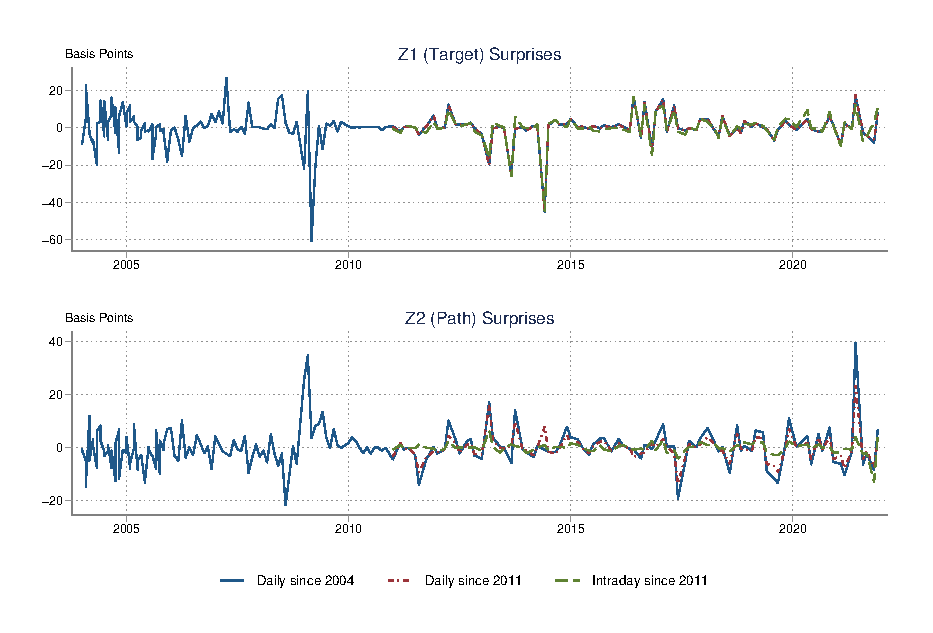
\includegraphics[width=1\textwidth,height=.4\textheight]{../Figures/factorslines.eps} \\
				\end{center}
				\vspace{-0.4cm}
				\fignotes{This figure compares the evolution of the \( \rtdone \) (target) and \( \rtdtwo \) (path) surprises obtained with daily data since 2004 (solid line) and 2011 (dash-dotted line), and with intraday data since 2011 (dashed line). The sample includes all regular monetary policy announcements up to \lastobs{}.}
			\end{minipage}
		\end{center}
	\end{figure}
\end{document}
% trim = {<left> <lower> <right> <upper>}
